\documentclass[notheorems,compress,mathserif,table]{beamer}

\useoutertheme{tree}
\usecolortheme{whale}      % Outer color themes, 其他选择: whale, seahorse, dolphin . 换一个编译看看有什么不同.
\usecolortheme{orchid}     % Inner color themes, 其他选择: lily, orchid
\useinnertheme[shadow]{rounded} % 对 box 的设置: 圆角、有阴影.
\setbeamercolor{sidebar}{bg=blue!50} % sidebar的颜色, 50%的蓝色.
%\setbeamercolor{background canvas}{bg=blue!9} % 背景色, 9%的蓝色. 去掉下一行, 试一试这个.
\setbeamertemplate{background canvas}[vertical shading][bottom=white,top=structure.fg!25] %%背景色, 上25%的蓝, 过渡到下白.
\usefonttheme{serif}  % 字体. 个人偏好有轮廓的字体. 去掉这个设置编译, 就看到不同了.
\setbeamertemplate{navigation symbols}{}   %% 去掉页面下方默认的导航条.
%%------------------------常用宏包---------------------------------------------------------------------
%%注意, beamer 会默认使用下列宏包: amsthm, graphicx, hyperref, color, xcolor, 等等
%\usepackage{CJK}
\usepackage{ctex}
\usepackage{amsmath,amsthm,amsfonts,amssymb,bm}
\usepackage{mathrsfs}
\usepackage{subfigure} %%图形或表格并排排列
\usepackage{xmpmulti}  %%支持文中的 \multiinclude 等命令, 使 mp 文件逐帧出现. 具体讨论见 beamer 手册.
\usepackage{colortbl,dcolumn}     %% 彩色表格
%\logo{
\includegraphics[height=0.09\textwidth]{ajln.jpg}}   %左上角科大logo
%%%%%%%%%%%%%%%%%%%%%%%%%%%%%%%%%%%%%%重定义字体、字号命令 %%%%%%%%%%%%%%%%%%%%%%%%%%%%%%%%%%%%%%%%%%%%%%
%\newcommand{\songti}{\CJKfamily{song}}        % 宋体
%\newcommand{\fangsong}{\CJKfamily{fs}}        % 仿宋体
%\newcommand{\kaishu}{\CJKfamily{kai}}         % 楷体
%\newcommand{\heiti}{\CJKfamily{hei}}          % 黑体
%\newcommand{\lishu}{\CJKfamily{li}}           % 隶书
\newcommand{\youyuang}{\CJKfamily{you}}       % 幼圆
\newcommand{\sanhao}{\fontsize{16pt}{\baselineskip}\selectfont}     % 字号设置
\newcommand{\sihao}{\fontsize{14pt}{\baselineskip}\selectfont}      % 字号设置
\newcommand{\xiaosihao}{\fontsize{12pt}{\baselineskip}\selectfont}  % 字号设置
\newcommand{\wuhao}{\fontsize{10.5pt}{\baselineskip}\selectfont}    % 字号设置
\newcommand{\xiaowuhao}{\fontsize{9pt}{\baselineskip}\selectfont}   % 字号设置
\newcommand{\liuhao}{\fontsize{7.875pt}{\baselineskip}\selectfont}  % 字号设置
\newcommand{\qihao}{\fontsize{5.25pt}{\baselineskip}\selectfont}    % 字号设置
%%%%%%%%%%%%%%%%%%%%%%%%%%%%%%%%%%%%%%%%%%%%%%%%%%%%%%%%%%%%%%%%%%%%%%%%%%%%%%%%%%%%%%%%%%%%%%%%%%%%%%%%
%%----------------------- Theorems ---------------------------------------------------------------------
\newtheorem{theorem}{定理}
\newtheorem{definition}{定义}
\newtheorem{lemma}{引理}
\newtheorem{example}{例题}
\newtheorem{answer}{解:}
\newtheorem{dablock}{}
\newtheorem{jytg}{提纲}
\newtheorem{daproof}{证明}
\newtheorem{explain}{说明}
\newtheorem{summary}{小结}

\newtheorem{zhuyi}{注意}
\newtheorem{zhu}{注:}
\newtheorem{shuoming}{说明}
\newtheorem{wenti}{问题}
\newtheorem{jielun}{结论}
\newtheorem{yinli}{引理}
%%----------------------------------------------------------------------------------------------------
\title{\heiti 第3章\quad 离散傅里叶变换}
\author[\textcolor{blue}]{{\sihao\kaishu  笪邦友}}
\institute{\sihao\lishu  \textcolor{violet}{中南民族大学~~ 电子信息工程学院}}
\date{\fangsong\today} 

\begin{document}
	%  \begin{CJK*}{GBK}{kai}
	\kaishu
	\frame{ \titlepage }
	%%---------------------------------------------------------------------------------------------------
	\section*{目录}
	\frame{\kaishu\frametitle{\kaishu 目录}\tableofcontents}
	\section*{前言}
	%%%%%%%%%%%%%%%%%%%%%%%%%%%%%%%%%%%%%%%%%%%%%%%%%%%%%%%%%%%%%%%%%%%%%%%%%%%%%%%%%%%%%%%%%%%%%%
%%% Local Variables:
%%% mode: latex
%%% TeX-master: t
%%% End:


\section{DFT的定义和物理意义}

\subsection{DFT的定义}
%
%
\begin{frame}[shrink]\frametitle{DFT的定义}%[allowframebreaks][shrink]
\begin{definition}
设有限长序列$x(n)$长度为$M$,则其$N$点$DFT$可定义为:
$$X(k) = DFT\big[x(n)\big] =  \sum_{n=0}^{N-1}x(n)e^{-j\frac{2\pi}{N}kn}  \quad\quad\quad (0 \leq k \leq N-1)$$
\end{definition}
\begin{zhu}
\begin{enumerate}
	\item [(1)]   式中$ M $为信号$ x(n) $的长度,$ N $为DFT变换区间长度,此处需要$ N\geq M $。
	\item [(2)]
\end{enumerate}
\end{zhu}

\end{frame}




\begin{frame}[shrink]\frametitle{DFT的定义}%[allowframebreaks][shrink]
    其反变换定义为:
    $$x(n) = IDFT[X(k)] =   \frac{1}{N}\sum_{k=0}^{N-1}X(k)e^{j\frac{2\pi}{N}kn} \quad\quad (0 \leq n \leq N-1)$$
    \begin{equation*}
           \left\{ \begin{aligned}
               X(k) &=  \sum_{n=0}^{N-1}x(n)e^{-j\frac{2\pi}{N}kn}  \quad\quad\quad (0 \leq k \leq N-1) \\
               x(n) &=   \frac{1}{N}\sum_{k=0}^{N-1}X(k)e^{j\frac{2\pi}{N}kn} \quad\quad (0 \leq n \leq N-1)
           \end{aligned} \right.
    \end{equation*}
\end{frame}




\begin{frame}[shrink]\frametitle{求反变换}%[allowframebreaks][shrink]
问题在于求反变换:
    $$x(n) =   \frac{1}{N}\sum_{k=0}^{N-1}X(k)e^{j\frac{2\pi}{N}kn} \quad\quad (0 \leq n \leq N-1)$$
\textbf{    证明:}  从右到左,将$X(k)$的表达式代入可得:
\begin{equation*}
\begin{split}
    %X(k) &=  \sum_{n=0}^{N-1}x(n)e^{-j\frac{2\pi}{N}kn}  \quad\quad\quad (0 \leq k \leq N-1) \\
\frac{1}{N}\sum_{k=0}^{N-1}X(k)e^{j\frac{2\pi}{N}kn}
    &= \frac{1}{N}\sum_{k=0}^{N-1}\left[\sum_{m=0}^{N-1}x(m)e^{-j\frac{2\pi}{N}km}\right]e^{j\frac{2\pi}{N}kn}   \\
    &=  \frac{1}{N}\sum_{m=0}^{N-1}x(m)\left[\sum_{k=0}^{N-1}e^{-j\frac{2\pi}{N}(m-n)k}\right]
\end{split}
\end{equation*}

\begin{equation*}
\mbox{而:\quad}    \sum_{k=0}^{N-1}e^{-j\frac{2\pi}{N}(m-n)k} =
        \left\{\begin{array}{r@{,\quad}l}
        N  & m-n =l\cdot N \quad\quad  l\in Z\\
        0     &\mbox{其他}
    \end{array} \right.
\end{equation*}


\end{frame}







\begin{frame}[shrink]\frametitle{求反变换}%[allowframebreaks][shrink]
因为$0\leqslant m \leqslant N-1$,$0\leqslant n \leqslant N-1$,
$$\therefore \quad\quad  -(N-1)\leqslant m-n \leqslant N-1$$

只有当$m-n=0$,即$m=n$时,有:
$$\sum_{k=0}^{N-1}e^{-j\frac{2\pi}{N}(m-n)k} = N$$


$$\therefore \quad\quad  \frac{1}{N}\sum_{m=0}^{N-1}x(m)\left[\sum_{k=0}^{N-1}e^{-j\frac{2\pi}{N}(m-n)k}\right]
 = \frac{1}{N}\cdot N \cdot x(n) = x(n)$$

$$\mbox{即:}\quad x(n) =   \frac{1}{N}\sum_{k=0}^{N-1}X(k)e^{j\frac{2\pi}{N}kn} \quad\quad (0 \leq n \leq N-1) $$
\end{frame}


\begin{frame}[shrink]\frametitle{求反变换}%[allowframebreaks][shrink]
记$W_N = e^{-j\frac{2\pi}{N}}$,则有:
    \begin{equation*}
           \left\{ \begin{aligned}
               X(k) &=  DFT[x(n)]\quad = \sum_{n=0}^{N-1}x(n) W_N^{kn} \quad\quad\quad (0 \leq k \leq N-1) \\
               x(n) &= IDFT[X(k)] = \frac{1}{N}\sum_{k=0}^{N-1}X(k)W_N^{-kn} \quad\quad (0 \leq n \leq N-1)
           \end{aligned} \right.
    \end{equation*}
\end{frame}
%




\subsection{DFT和Z变换的关系}

\begin{frame}\frametitle{DFT和Z变换的关系}%[allowframebreaks][shrink]
%$$ X(z) = \sum_{n=-\infty}^{\infty}x(n)z^{-n}\quad\quad\quad\quad\quad\quad\quad\quad\quad $$
我们知道:
\begin{equation*}
\begin{split}
                X(z) &= \sum_{n=-\infty}^{\infty}x(n)z^{-n}\qquad\qquad\qquad\qquad\qquad\qquad\qquad\qquad\qquad \\
\mbox{而}\quad  X(k) &= \sum_{n=0}^{N-1}x(n)e^{-j\frac{2\pi}{N}kn}
                      = \sum_{n=-\infty}^{\infty}x(n)e^{-j\frac{2\pi}{N}kn}\\
                     &= \left[\sum_{n=-\infty}^{\infty}x(n) z^{-n}\right]_{z = e^{-j\frac{2\pi}{N}k}} =X(z)\Big|_{z = e^{j\frac{2\pi}{N}k}}   \\
\therefore  X(k)     &= X(z)\Big|_{z = e^{j\frac{2\pi}{N}k}} \quad\quad\quad 0 \leq k \leq N-1
\end{split}
\end{equation*}
即,$x(n)$的$N$点$DFT$是其$Z$变换$X(z)$在单位圆上的$N$点等间隔采样。
\end{frame}

%%%%%%%%%%%%%%%%%%%%%%%%%%%%%%%%%%%%%%%%%%%%%%%%%%%%%%%%%%%%%%%%%%%%%%%%%%%%%%%%%%%%%%%%%%%%%%



%%%%%%%%%%%%%%%%%%%%%%%%%%%%%%%%%%%%%%%%%%%%%%%%%%%%%%%%%%%%%%%%%%%%%%%%%%%%%%%%%%%%%%%%%%%%%%%
%\begin{frame}[shrink]\frametitle{title}%[allowframebreaks][shrink]


\subsection{DFT和傅里叶变换的关系}

\begin{frame}[shrink]\frametitle{DFT和傅里叶变换的关系}%[allowframebreaks][shrink]
%$$ X(e^{j\omega}) = \sum_{n=-\infty}^{\infty}x(n)e^{-j\omega n}\qquad\qquad\quad\quad\quad\quad\quad\quad\quad $$
我们知道序列$x(n)$傅里叶变换为:
\begin{equation*}
\begin{split}
 X(e^{j\omega}) &= \sum_{n=-\infty}^{\infty}x(n)e^{-j\omega n}\qquad\qquad\qquad\qquad\qquad\qquad\qquad\qquad\qquad\\
\mbox{而}\qquad    X(k) &= \sum_{n=0}^{N-1}x(n)e^{-j\frac{2\pi}{N}kn}
          = \sum_{n=-\infty}^{\infty}x(n)e^{-j\frac{2\pi}{N}kn}\\
         &= \left[\sum_{n=-\infty}^{\infty}x(n) e^{-j\omega n}\right]_{\omega = \frac{2\pi}{N}k}   \\
\therefore \qquad    X(k) &= X(e^{j\omega})\Big|_{\omega = \frac{2\pi}{N}k} \qquad\qquad\qquad   (0 \leq k \leq N-1)
\end{split}
\end{equation*}

即,$x(n)$的$N$点$DFT$是其傅里叶变换$X(e^{j\omega})$在$\omega$ 轴上区间$[0,2\pi]$上的N点等间隔采样。这也是$DFT$的物理意义。
\end{frame}

\begin{frame}[shrink]\frametitle{例题}%[allowframebreaks][shrink]

由此可见,$DFT$变换区间长度不同,$X(k)$在傅里叶变换$X(e^{j\omega})$ 的区间$[0,2\pi]$上的采样点数不同,其$DFT$ 的结果也不同
\begin{example}
设$x(n)=R_4(n)$,求$x(n)$的4点,8 点,16点DFT。
\end{example}
\quad\newline\newline\newline\newline\newline\newline\newline\newline\newline\quad


\end{frame}

\begin{frame}\frametitle{DFT的重要性}%[allowframebreaks][shrink]

{\heiti $DFT$的重要性表现于:\par\quad}
\newline
其实质是有限长序列$x(n)$的傅里叶变换$X(e^{j\omega})$的有限点离散采样,实现了频域离散化,从而可在频域采用数值计算方法进行数字信号处理。
$$X(k) = \sum_{n=0}^{N-1}x(n) W_N^{kn} \quad\quad\quad (0 \leq k \leq N-1) $$
\end{frame}

%%%%%%%%%%%%%%%%%%%%%%%%%%%%%%%%%%%%%%%%%%%%%%%%%%%%%%%%%%%%%%%%%%%%%%%%%%%%%%%%%%%%%%%%%%%%%%%



%%%%%%%%%%%%%%%%%%%%%%%%%%%%%%%%%%%%%%%%%%%%%%%%%%%%%%%%%%%%%%%%%%%%%%%%%%%%%%%%%%%%%%%%%%%%%%%%

%%

\subsection{DFT的隐含周期性}

\begin{frame}[shrink]\frametitle{DFT的隐含周期性}%[allowframebreaks][shrink]
$$X(k) = \sum_{n=0}^{N-1}x(n) W_N^{kn} \quad\quad\quad (0 \leq k \leq N-1) $$
\textbf{一、分析}:
\begin{enumerate}
  \item 从公式上看,$0 \leq k \leq N-1$,$X(k)$是有限长序列,不可能是周期序列。
  \item 从公式形式上看,$X(k)$的表达式是周期为N的周期函数。
\end{enumerate}

%\textbf{二、几个约定的符号}
%
%设$\tilde{x}(n)$是周期为N的周期序列,是$x(n)$的周期延拓,即
%\begin{equation*}
%    \left\{ \begin{aligned}
%    \tilde{x}(n)\mbox{是$x(n)$的周期延拓} \\
%    x(n)\mbox{是$\tilde{x}(n)$的主值序列}
%    \end{aligned} \right.
%\end{equation*}
\end{frame}
%



\begin{frame}[shrink]\frametitle{}%[allowframebreaks][shrink]
\textbf{二、几个约定的符号}

设$\tilde{x}(n)$是周期为N的周期序列,是$x(n)$的周期延拓,即
\begin{equation*}
    \left\{ \begin{aligned}
    \tilde{x}(n)\mbox{是$x(n)$的周期延拓} \\
    x(n)\mbox{是$\tilde{x}(n)$的主值序列}
    \end{aligned} \right.
\end{equation*}
记做:
$$  x(n) = \tilde{x}(n)\cdot R_N(n) \quad\quad\quad\quad\quad\quad\quad\quad\quad$$
$$  \tilde{x}(n)   = x((n))_N  \quad\quad\quad\quad\quad (\mbox{$n$对$N$求余})$$

例如: $$x((10))_8 = x(2) \quad\quad ((1))_8 = 1  \quad\quad ((16))_8 =0 $$

且有公式
$$\mbox{\quad\quad }   \underbrace{\tilde{x}(n)}_{-\infty\leq n\leq \infty} =
 \underbrace{\sum_{m=-\infty}^{\infty}x(n+mN)}_{0 \leq n\leq N-1}$$
\end{frame}






\begin{frame}[shrink]\frametitle{$DFT$和$DFS$的关系}%[allowframebreaks][shrink]
%\textbf{三、$DFT$和$DFS$的关系}

%$$\mbox{设:\quad} x(n)\longleftrightarrow X(k)\quad\quad\quad  \tilde{x}(n)\longleftrightarrow \tilde{X}(k)$$
$$\mbox{设:\quad} x(n)\longleftrightarrow X(k)  \qquad\qquad\qquad$$

$$\mbox{\qquad\quad}   \tilde{x}(n)\longleftrightarrow \tilde{X}(k)\qquad\qquad\qquad$$


则:
\begin{equation*}
    \left\{ \begin{aligned}
    X(k)         &=DFT[x(n)]        &= \sum_{n=0}^{N-1}x(n) e^{-j\frac{2\pi}{N}kn} \qquad (0 \leq k \leq N-1) \\
    \tilde{X}(k) &=DFS[\tilde{x}(n)]&= \sum_{n=0}^{N-1}\tilde{x}(n) e^{-j\frac{2\pi}{N}kn} \qquad (-\infty \leq k \leq \infty) \\
    \end{aligned} \right.
\end{equation*}

%显然:
%\begin{enumerate}
%  \item 公式完全一样
%  \item $X(k)$是$\tilde{X}(k)$的主值序列,即$X(k)=\tilde{X}(k)R_N(k)$。\par
%        周期序列$\tilde{x}(n)$的频谱完全由其DFS的系数$\tilde{X}(k)$确定,因此$X(k)$实际上是$x(n)$的周期延拓序列$\tilde{x}(n)$ 的频谱特性,这也是DFT 的第二种物理意义。
%\end{enumerate}
\end{frame}

\begin{frame}[shrink]\frametitle{}%[allowframebreaks][shrink]
\begin{equation*}
    \left\{ \begin{aligned}
    X(k)         &=DFT[x(n)]        &= \sum_{n=0}^{N-1}x(n) e^{-j\frac{2\pi}{N}kn} \quad (0 \leq k \leq N-1) \\
    \tilde{X}(k) &=DFS[\tilde{x}(n)]&= \sum_{n=0}^{N-1}\tilde{x}(n) e^{-j\frac{2\pi}{N}kn} \quad (-\infty \leq k \leq \infty) \\
    \end{aligned} \right.
\end{equation*}
显然:
\begin{enumerate}
  \item 公式完全一样
  \item $X(k)$是$\tilde{X}(k)$的主值序列,即$X(k)=\tilde{X}(k)R_N(k)$。\par
        周期序列$\tilde{x}(n)$的频谱完全由其DFS的系数$\tilde{X}(k)$确定,因此$X(k)$实际上是$x(n)$的周期延拓序列$\tilde{x}(n)$ 的频谱特性,这也是DFT 的第二种物理意义。
  \item 由$x(n)$得到$X(k)$的过程为:
            $$x(n)\quad \stackrel{\mbox{延拓}}{\longrightarrow}\quad  \tilde{x}(n)
            \quad \stackrel{DFS}{\longrightarrow}\quad \tilde{X}(k)
            \quad \stackrel{\mbox{取主值}}{\longrightarrow}\quad X(k)$$
\end{enumerate}
\end{frame}


\begin{frame}[shrink]\frametitle{$DFT$理论的近似性}%[allowframebreaks][shrink]
\textbf{$DFT$理论的近似性}
\begin{enumerate}
  \item DFT理论的前提是$x_a(t)$ 为有限长带限信号,即信号在时域为有限长,频域也为有限长。
  \item 实际中不存在这种信号,时域有限和频域有限是一对矛盾,不可能同时实现。时域上有限的信号,其频域信号必定无限长。
  \item 在工程实践中,时域有限信号容易得到,但其能量往往集中于低频段,频谱具有收敛性,在频率大于一定值后,其频谱分量近似为0了。通常可将其截断,从而得到有限长带限信号。
\end{enumerate}
\end{frame}
%%

\section{$DFT$的基本性质}

\subsection{线性性质}

%\begin{frame}[shrink]\frametitle{线性性质}%[allowframebreaks][shrink]
%
%\end{frame}


\subsection{循环移位性质}
\begin{frame}[shrink]\frametitle{序列的循环移位}%[allowframebreaks][shrink]
一、序列的循环移位

设$x(n)$长度为N,则:$y(n) = x((n+m))_N\cdot R_N(n)$称为$x(n)$ 的循环移位序列。


步骤
\begin{enumerate}
  \item 延拓 \quad \quad\quad \quad     $x(n)\longrightarrow \tilde{x}(n) = x((n))_N$
  \item 移位 \quad \quad \quad \quad    $\tilde{x}(n)\longrightarrow \tilde{x}(n+m) = x((n+m))_N$
  \item 取主值  \quad \quad \quad       $x((n+m))_N\cdot R_N(n)$
\end{enumerate}

\begin{example}
已知$x(n)$如图所示,
画出$x((n+2))_5 \cdot R_5(n)$。
\end{example}
\quad\newline\newline\newline\newline\quad
\end{frame}




\begin{frame}[shrink]\frametitle{时域循环移位定理}%[allowframebreaks][shrink]
\textbf{二、时域循环移位定理}

设有限长序列$x(n)$长度为N,$X(k)$为其N点DFT,则有:
$$x((n+m))_N\cdot R_N(n) \longleftrightarrow W_N^{-km}\cdot X(k)$$

\end{frame}

\begin{frame}[shrink]\frametitle{}%[allowframebreaks][shrink]
\textbf{证明:}  从左到右

$DFT\bigg[ x((n+m))_N R_N(n)\bigg]$
\begin{equation*}
\begin{split}
    \quad
         &= \sum_{n=0}^{N-1}\bigg[x((n+m))_N R_N(n)\bigg]W_N^{kn}
          = \sum_{n=0}^{N-1}\bigg[x((n+m))_N\bigg]W_N^{kn} \quad\mbox{(主值区间)}\quad\\
         &\quad  \mbox{令} n' =n+m,\mbox{则有:}  \\
         &= \sum_{n'=m}^{m+N-1}\bigg[x((n'))_N\bigg]W_N^{k(n'-m)}
          = W_N^{-km}\sum_{n'=m}^{m+N-1}\bigg[x((n'))_N\bigg]W_N^{kn'}\\
         &= W_N^{-km}\sum_{n'=0}^{N-1}\bigg[x((n'))_N\bigg]W_N^{kn'}\quad\mbox{(一个周期内求和相等)}\\
         &= W_N^{-km}\sum_{n'=0}^{N-1}x(n')W_N^{kn'}  \quad\quad\quad\quad\mbox{(主值区间)}\\
         &= W_N^{-km}X(k)
\end{split}
\end{equation*}
$$x((n+m))_N R_N(n) \longleftrightarrow W_N^{-km}X(k)$$

\end{frame}



\begin{frame}[shrink]\frametitle{频域循环移位定理}%[allowframebreaks][shrink]
三、频域循环移位定理

设有限长序列$x(n)$长度为N,$X(k)$为其N点DFT,则有:
$$W_N^{km}\cdot x(n) \longleftrightarrow X((k+m))_N\cdot R_N(k)$$


\end{frame}

\begin{frame}[shrink]\frametitle{}%[allowframebreaks][shrink]
\textbf{证明:}  从右到左

$IDFT\big[ X((k+m))_N R_N(k)\big]$
\begin{equation*}
\begin{split}
    \quad
         &= \frac{1}{N}\sum_{k=0}^{N-1}\bigg[X((k+m))_N R_N(k)\bigg]W_N^{-kn}
          = \frac{1}{N}\sum_{k=0}^{N-1}\bigg[X((k+m))_N \bigg]W_N^{-kn} \quad\mbox{(主值区间)}\quad\\
         &\quad  \quad\quad\quad\quad\mbox{令} k' =k+m,\mbox{则有:}  \\
         &= \frac{1}{N}\sum_{k'=m}^{m+N-1}\bigg[X((k'))_N\bigg]W_N^{-k'n}W_N^{km}\\
         &= W_N^{km}\cdot\frac{1}{N}\sum_{k'=m}^{m+N-1}\bigg[X((k'))_N\bigg]W_N^{-k'n} \qquad \\
         &= W_N^{km}\cdot\frac{1}{N}\sum_{k'=0}^{N-1}\bigg[X((k'))_N\bigg]W_N^{-k'n}\quad\mbox{(一个周期内求和相等)}\\
         &= W_N^{km}\cdot\frac{1}{N}\sum_{k'=0}^{N-1}X(k') W_N^{-kn'}  \quad\quad\quad\quad\mbox{(主值区间)}\\
         &= W_N^{km}\cdot x(n)
\end{split}
\end{equation*}

$$\mbox{即: \quad\quad }W_N^{km}\cdot x(n) \longleftrightarrow X((k+m))_N\cdot R_N(k)$$

\end{frame}


\subsection{循环卷积定理}

\begin{frame}[shrink]\frametitle{循环卷积的定义}%[allowframebreaks][shrink]
\textbf{一、循环卷积的定义}
\begin{definition}
设有限长序列$x(n)$和$h(n)$的长度分别为$M$和$N$。则$x(n)$和$h(n)$的$L$ 点循环卷积定义为:
\begin{equation*}
\begin{split}
  y_c(n) &= x(n) \otimes h(n) \\
         &= \bigg[ \sum_{m=0}^{L-1} h(m) x((n-m))_L \bigg] R_L(n)
\end{split}
\end{equation*}
式中L称为循环卷积区间长度,且有$L\geq \{N,M\}$。
\end{definition}
\begin{enumerate}
  \item 延拓 \quad\quad\quad\quad $x(n)\longrightarrow \tilde{x}(n)=x((n))_L$
  \item 线性卷积  \quad\quad $h(n)* \tilde{x}(n)$
  \item 取主值
\end{enumerate}
\end{frame}


\begin{frame}[shrink]\frametitle{循环卷积计算示例}%[allowframebreaks][shrink]
\begin{example}
设$h(n)=R_4(n)$,$x(n) = R_4(n-2)$,求其循环卷积,设$L=8$。
\end{example}
\end{frame}
%
%
%
\begin{frame}[shrink]\frametitle{时域循环卷积定理}%[allowframebreaks][shrink]
\textbf{二、时域循环卷积定理}
\quad\newline\quad
\begin{theorem}
设长度均为N的有限长序列$x_1(n)\leftrightarrow X_1(k)$,$x_2(n)\leftrightarrow X_2(k)$,则有:
$$x_1(n)\otimes x_2(n) \longleftrightarrow X_1(k)\cdot X_2(k) \quad\quad (\mbox{$N$点循环卷积})$$
\end{theorem}
\end{frame}

\begin{frame}[shrink]\frametitle{}%[allowframebreaks][shrink]
\textbf{证明:}

$DFT\big[ x_1(n)\otimes x_2(n)\big]$
\begin{equation*}
\begin{split}
    \quad
         &= \sum_{n=0}^{N-1}\bigg[x_1(n)\otimes x_2(n)\bigg]W_N^{kn} \\
         &= \sum_{n=0}^{N-1}\left[\sum_{m=0}^{N-1}x_1(m) x_2((n-m))_N R_N(n) \right] W_N^{kn}   \\
         &= \sum_{m=0}^{N-1}x_1(m)\left[ \sum_{n=0}^{N-1} x_2((n-m))_N R_N(n) W_N^{kn} \right]   \\
         &= \sum_{m=0}^{N-1}x_1(m) DFT\bigg[  x_2((n-m))_N R_N(n) \bigg]  \quad   \\
         &= \sum_{m=0}^{N-1}x_1(m)W_N^{km} X_2(k)  \;\qquad\qquad      \\
         &= X_1(k)\cdot X_2(k)
\end{split}
\end{equation*}
注意时域循环移位性质:
$$x((n+m))R_N(n)\leftrightarrow W_N^{-km}X(k)  \qquad\qquad   x((n-m))R_N(n)\leftrightarrow W_N^{km}X(k) $$
\end{frame}
%
%





\begin{frame}[shrink]\frametitle{频域循环卷积定理}%[allowframebreaks][shrink]
\textbf{三、频域循环卷积定理}
\quad\newline\quad
\begin{theorem}
设长度均为N的有限长序列$x_1(n)\leftrightarrow X_1(k)$,$x_2(n)\leftrightarrow X_2(k)$,则有:
$$x_1(n)\cdot x_2(n)\longleftrightarrow\frac{1}{N}X_1(k)\otimes X_2(k)\quad\quad(\mbox{$N$点循环卷积})$$
\end{theorem}
\end{frame}





\begin{frame}[shrink]\frametitle{}%[allowframebreaks][shrink]
\textbf{证明:}

$IDFT\big[ \frac{1}{N}X_1(k) \otimes X_2(k)\big]$
\begin{equation*}
\begin{split}
    \quad
         &= \frac{1}{N}\sum_{k=0}^{N-1}\bigg[ \frac{1}{N}X_1(k) \otimes X_2(k) \bigg]W_N^{-kn} \\
         &= \frac{1}{N}\sum_{k=0}^{N-1}\left[\frac{1}{N}\sum_{m=0}^{N-1}X_1(m) X_2((k-m))_N \right] R_N(k) W_N^{-kn}   \\
         &= \frac{1}{N}\sum_{m=0}^{N-1}X_1(m)\left[ \frac{1}{N}\sum_{k=0}^{N-1} X_2((k-m))_N R_N(k) W_N^{-kn} \right]   \\
         &= \frac{1}{N}\sum_{m=0}^{N-1}X_1(m)\cdot IDFT\Big[  X_2((k-m))_N R_N(k) \Big]  \quad \\
                %\Big(W_N^{km}\cdot x(n) \longleftrightarrow X((k+m))_N\cdot R_N(k)\Big)\\
         &= \Big[\frac{1}{N}\sum_{m=0}^{N-1} X_1(m)W_N^{-km}\Big] x_2(n) \\
                %\quad\quad\quad\quad\quad\quad\quad\quad \Big(W_N^{-km}\cdot x(n) \longleftrightarrow X((k-m))_N\cdot R_N(k)\Big)    \\
         &= x_1(n)\cdot x_2(n)
\end{split}
\end{equation*}
注意频域移位性质:
$$W_N^{km}\cdot x(n) \longleftrightarrow X((k+m))_N\cdot R_N(k)  \qquad\qquad
  W_N^{-km}\cdot x(n) \longleftrightarrow X((k-m))_N\cdot R_N(k) $$
\end{frame}
%
\subsection{复共轭序列的DFT}


\begin{frame}[shrink]\frametitle{复共轭序列的DFT}%[allowframebreaks][shrink]
\begin{theorem}
设长度为$N$的有限长序列$x(n)\leftrightarrow X(k)$,且令$X(N)=X(0)$,则有:
$$\qquad x^*(n) \quad \longleftrightarrow  X^*(N-k) \qquad\quad \big(0\leq k\leq N-1\big) \quad$$
$$ x^*(N-n) \longleftrightarrow  \quad X^*(k) \qquad\qquad \big(0\leq k\leq N-1\big) $$
\end{theorem}
\begin{equation*}
\begin{split}
    X(k)     &= \sum_{n=0}^{N-1}x(n)W_N^{kn}    \\
    X(N-k)   &= \sum_{n=0}^{N-1}x(n)W_N^{(N-k)n}
              = \sum_{n=0}^{N-1}x(n)W_N^{-kn}W_N^{Nn}
              = \sum_{n=0}^{N-1}x(n)W_N^{-kn}       \\%    \qquad\qquad\big(W_N^{Nn} =1\big)   \\
    X^*(N-k) &= \left[\sum_{n=0}^{N-1}x(n)W_N^{-kn}\right]^*  = \sum_{n=0}^{N-1}x^*(n)W_N^{kn} = DFT\big[x^*(n)\big]
\end{split}
\end{equation*}
\end{frame}


\begin{frame}[shrink]\frametitle{复共轭序列的DFT}%[allowframebreaks][shrink]
$$\mbox{同理可证: \quad\quad }  x^*(N-n) \longleftrightarrow  X^*(k) \quad\quad \big(0\leq k\leq N-1\big) $$
$DFT\Big[x^*(N-n)\Big]$
\begin{equation*}
\begin{split}
\quad   &= \sum_{n=0}^{N-1}x^*(N-n)W_N^{kn}  \quad\quad\quad\quad\mbox{令}m=N-n  \\
        &= \sum_{m=0}^{N-1}x^*(m)W_N^{k(N-m)}
        =  \sum_{m=0}^{N-1}x^*(m)W_N^{-km}W_N^{kN}   \\
        &= \sum_{m=0}^{N-1}x^*(m)W_N^{-km}     \quad\quad \mbox{因为}\big(W_N^{kN} =1\big)   \\
        &= \left[\sum_{m=0}^{N-1}x(m)W_N^{km}\right]^*  = X^*(k)
\end{split}
\end{equation*}
\end{frame}
%
%

\subsection{DFT的共轭对称性}



\begin{frame}[shrink]\frametitle{DFT的共轭对称性}%[allowframebreaks][shrink]
\textbf{一、复习一下离散序列的分解}
\begin{dablock}
任何离散序列可分解为共轭对称序列和共轭反对称序列之和,也能分解为实数部分序列和虚数部分序列之和。
\end{dablock}



%\parbox{0.1cm}{\Bigg\{ }\hfill
%\parbox{5cm}{\begin{eqnarray*}
%x_{e}(n) &=& \frac{1}{2}\big[x(n) + x^{*}(-n)\big]\\
%x_{o}(n) &=& \frac{1}{2}\big[x(n) - x^{*}(-n)\big]
%\end{eqnarray*} }\hfill
%\parbox{5cm}{\begin{eqnarray*}
%x_{r}(n)  &=& \frac{1}{2}\big[x(n) + x^{*}(n)\big]\\
%jx_{i}(n) &=& \frac{1}{2}\big[x(n) - x^{*}(n)\big]
%\end{eqnarray*} }
%%---------------------------------------------------------------------------------

\begin{equation*} %\label{fol2218}
\left\{ \begin{aligned}
    x_{e}(n) &= \frac{1}{2}\big[x(n) + x^{*}(-n)\big]  \quad\quad\quad\quad\quad\quad\quad\\
    x_{o}(n) &= \frac{1}{2}\big[x(n) - x^{*}(-n)\big]
\end{aligned} \right.
\end{equation*}

\begin{equation*} %\label{fol2218}
\left\{ \begin{aligned}
    x_{r}(n)  &= \frac{1}{2}\big[x(n) + x^{*}(n)\big]   \quad\quad\quad\quad\quad\quad\quad\\
    jx_{i}(n) &= \frac{1}{2}\big[x(n) - x^{*}(n)\big]
\end{aligned} \right.
\end{equation*}
\end{frame}


\begin{frame}[shrink]\frametitle{有限长序列的对称性}%[allowframebreaks][shrink]
\textbf{二、$DFT$中也存在类似的对称性,}
\newline
设$x(n)$为长度为$N$的有限长序列。
\newline
$1^o$ 记号:
\begin{equation*} %\label{fol2218}
\left\{ \begin{aligned}
    x_{ep}(n) &: \mbox{有限长共轭对称序列}  \quad\quad\quad\quad\quad\quad\quad\quad\quad\\
    x_{op}(n) &: \mbox{有限长共轭反对称序列}
\end{aligned} \right.
\end{equation*}

$2^o$ 定义:
\begin{equation*} %\label{fol2218}
\left\{ \begin{aligned}
    x_{ep}(n) &= \quad x_{ep}^*(N-n)  \quad\quad\mbox{对比:}  x_{e}(n) = x_{e}^*(-n) \quad\quad\\
    x_{op}(n) &= -x_{op}^*(N-n)       \:\quad\quad\mbox{对比:}       x_{o}(n) = -x_{o}^*(-n)
\end{aligned} \right.
\end{equation*}
\end{frame}






\begin{frame}[shrink]\frametitle{其实质为有限长序列$x(n)$关于$\frac{N}{2}$对称}%[allowframebreaks][shrink]
\begin{dablock}
其实质为有限长序列$x(n)$关于$\frac{N}{2}$对称。
\end{dablock}
如$N$为偶数,令$n=\frac{N}{2}-n_0$,可得:
\begin{equation*} %\label{fol2218}
\left\{ \begin{aligned}
    x_{ep}\big(\frac{N}{2}-n_0\big) &= \quad x_{ep}^*\big(\frac{N}{2}+n_0\big)  \quad\quad\quad\quad\quad\quad\quad\quad\quad\quad\\
    x_{op}\big(\frac{N}{2}-n_0\big) &= -x_{op}^*\big(\frac{N}{2}+n_0\big)
\end{aligned} \right.
\end{equation*}
\end{frame}


\begin{frame}[shrink]\frametitle{ 有限长序列的分解}%[allowframebreaks][shrink]
$3^o$ 讨论:
\begin{enumerate}
  \item 有限长序列可分解为共轭对称序列和共轭反对称序列。
\begin{equation*}
        \begin{split}
        \mbox{令} : \quad\quad\quad\quad x(n)  &=  x_{ep}(n) + x_{op}(n)   \\
        \mbox{则} : \quad   x^*(N-n)           &= x_{ep}^*(N-n) + x_{op}^*(N-n)  \quad\quad\quad\quad\quad\quad\quad\quad  \\
                                                &= x_{ep}(n) - x_{op}(n)
        \end{split}
        \end{equation*}

        联立求解可得:
        \begin{equation*} %\label{fol2218}
        \left\{ \begin{aligned}
            x_{ep}(n) &= \frac{1}{2}\big[x(n) + x^{*}(N-n)\big]  \quad\quad\quad\quad\quad\quad\quad\\
            x_{op}(n) &= \frac{1}{2}\big[x(n) - x^{*}(N-n)\big]
        \end{aligned} \right.
        \end{equation*}
        
\item 同样,有限长序列可分解为实数部分序列和虚数部分序列。
        \begin{equation*} %\label{fol2218}
        \left\{ \begin{aligned}
            x_{r}(n)  &= \frac{1}{2}\big[x(n) + x^{*}(n)\big]   \quad\quad\quad\quad\quad\quad\quad\\
            jx_{i}(n) &= \frac{1}{2}\big[x(n) - x^{*}(n)\big]
        \end{aligned} \right.
        \end{equation*}
\end{enumerate}        
\end{frame}



%\begin{frame}[shrink]\frametitle{title}%[allowframebreaks][shrink]
%
%
%        同样,有限长序列可分解为实数部分序列和虚数部分序列。
%        \begin{equation*} %\label{fol2218}
%        \left\{ \begin{aligned}
%            x_{r}(n)  &= \frac{1}{2}\big[x(n) + x^{*}(n)\big]   \quad\quad\quad\quad\quad\quad\quad\\
%            jx_{i}(n) &= \frac{1}{2}\big[x(n) - x^{*}(n)\big]
%        \end{aligned} \right.
%        \end{equation*}
%
%\end{frame}

\begin{frame}[shrink]\frametitle{对称性讨论—实部序列和虚部部分序列的DFT}%[allowframebreaks][shrink]
        (1)  $\mbox{设: \quad}  x(n) = x_r(n) +j x_i(n) \quad\quad X(k) = X_{ep}(k) + X_{op}(k)\quad$
        $$\quad\mbox{则: \quad}\quad x_r(n)\leftrightarrow X_{ep}(k) \quad\quad\quad\quad\quad jx_i(n)\leftrightarrow X_{op}(k)\quad\quad\quad$$

        证:%\vspace{-0.5cm}
        \begin{enumerate}
          \item [(a)] \qquad $x_r(n)\leftrightarrow X_{ep}(k)$
                \begin{equation*}
                \begin{split}
                \because \quad  x_{r}(n)  &= \frac{1}{2}\big[x(n) + x^{*}(n)\big]  \quad\quad\big(x^*(n)\leftrightarrow X^*(N-k)\big)\\
                    DFT\big[x_{r}(n)\big] &= \frac{1}{2}\big[X(k) + X^{*}(N-k)\big]  = X_{ep}(k)
                \end{split}
                \end{equation*}
\item  [(b)] \qquad $jx_i(n)\leftrightarrow X_{op}(k)$
        \begin{equation*}
        \begin{split}
        \because \quad  jx_{i}(n) &= \frac{1}{2}\big[x(n) - x^{*}(n)\big]  \quad\quad\big(x^*(n)\leftrightarrow X^*(N-k)\big)\\
            DFT\big[jx_{i}(n)\big] &= \frac{1}{2}\big[X(k) - X^{*}(N-k)\big]  = X_{op}(k)
        \end{split}
        \end{equation*}
\end{enumerate}        
\end{frame}


\begin{frame}[shrink]\frametitle{对称性讨论—共轭对称与共轭反对称序列的DFT}%[allowframebreaks][shrink]
        (2)  $\mbox{设: \quad}  x(n) = x_{ep}(n) +  x_{op}(n) \quad\quad X(k) = X_{R}(k) + jX_{I}(k)\quad$
        $$\quad\mbox{则: \quad}\quad x_{ep}(n)\leftrightarrow X_{R}(k) \quad\quad\quad\quad\quad x_{op}(n)\leftrightarrow jX_{I}(k)\quad\quad\quad$$

        证: %\vspace{-0.5cm}
        \begin{enumerate}
          \item [(a)] $\quad x_{ep}(n)\leftrightarrow X_{R}(k)$
            \begin{equation*}
            \begin{split}
            \because \quad  x_{ep}(n)  &= \frac{1}{2}\big[x(n) + x^{*}(N-n)\big]  \quad\quad\big(x^*(N-n)\leftrightarrow X^*(k)\big)\\
                DFT\big[x_{ep}(n)\big] &= \frac{1}{2}\bigg[X(k) + X^{*}(k)\bigg]  = X_{R}(k)
            \end{split}
            \end{equation*}
        \item [(b)]   $\quad x_{op}(n)\leftrightarrow jX_{I}(k)$
            \begin{equation*}
            \begin{split}
           \because \quad  x_{op}(n)  &= \frac{1}{2}\bigg[x(n) - x^{*}(N-n)\bigg]     \quad\quad\big(x^*(N-n)\leftrightarrow X^*(k)\big)\\
                DFT\big[x_{op}(n)\big] &= \frac{1}{2}\bigg[X(k) - X^{*}(k)\bigg]  = jX_{I}(k)
            \end{split}
            \end{equation*}
\end{enumerate}
\end{frame}






\begin{frame}[shrink]\frametitle{有限长序列对称性结论}%[allowframebreaks][shrink]
\begin{jielun}
\begin{enumerate}
	\item [(1)]  一个域的共轭对称序列对应另一个域的实数部分序列,反之亦然。
   	\item [(2)]  一个域的共轭反对称序列对应另一个域的虚数部分序列,反之亦然。
\end{enumerate}
\end{jielun}
\end{frame}


\begin{frame}[allowframebreaks]\frametitle{实序列$x(n)$的对称性讨论}%[allowframebreaks][shrink]
\begin{dablock}
  % 实序列$x(n)$的对称性讨论
      设$x(n)\leftrightarrow X)k)$,因为$x(n)\in R$,\quad\newline\newline\quad
      则有$X(k)=X^*(N-k)$, 即$X(k)$ 为共轭对称序列。
\end{dablock}

      \begin{enumerate}
        \item  若$x(n) = x(N-n)$, 即$x(n)$ 为实偶序列。则有:
        \begin{equation*} %\label{fol2218}
            \left\{ \begin{aligned}
                x(n)\mbox{为实序列} \qquad   &\rightarrow  \quad X(k)\mbox{为共轭对称序列}\newline  \\
                                    \qquad   &\qquad \qquad\mbox{即:} X(k)=X^*(N-k) \quad\quad\quad\quad\quad\quad\quad\\
                x(n)\mbox{为实偶序列} \quad   &\rightarrow \quad X(k)\mbox{为实数序列}\\
            \end{aligned} \right.
        \end{equation*}
        则有$X(k)=X^*(N-k) = X(N-k)$,也就是说$X(k)$也是实偶序列。
        \newpage
        \item  若$x(n) = -x(N-n)$,即$x(n)$ 为实奇序列。则有:
        \begin{equation*} %\label{fol2218}
            \left\{ \begin{aligned}
                x(n)\mbox{为实序列}   \qquad   &\rightarrow \quad X(k)\mbox{为共轭对称序列}  \quad\quad\quad\quad\quad\quad\quad\\
                                      \qquad   &\qquad \qquad\mbox{即:}X(k)=X^*(N-k)  \quad\quad\quad\quad\quad\quad\quad\\
                x(n)\mbox{为实奇序列}  \quad  &\rightarrow \quad X(k)\mbox{为纯虚数序列}\\
            \end{aligned} \right.
        \end{equation*}
        则有$X(k)=X^*(N-k) = -X(N-k)$,也就是说$X(k)$是纯虚奇对称序列。
      \end{enumerate}

\end{frame}


\begin{frame}[allowframebreaks]\frametitle{ 应用举例:(实序列$DFT$计算量减半)}%[allowframebreaks][shrink]

      \begin{enumerate}
        \item [例1] 如$N=8$,求$X(k)$。 \quad\newline\newline\quad
              利用对称性,有$X(k)=X^*(N-k)$,\quad\newline\newline\quad
              只需求$X(0)$,$X(1)$,$X(2)$,$X(3)$,$X(4)$,则有:
              $$X(5)=X^*(3),\quad\quad X(6)=X^*(2),\quad\quad X(7)= X^*(1)$$
        \newpage
        \item [例2] 计算一个$N$ 点$DFT$,同时得到两个实序列的$N$点$DFT$。
        
        \quad\newline\quad
              设$x_1(n)$,$x_2(n)$ 是两个长度为$N$的实序列。
              $$\mbox{令 :}\qquad\qquad x(n) = x_1(n)+jx_2(n)\quad\:
              \qquad\qquad\qquad\qquad$$
              $$\mbox{则 :}\qquad\qquad X(k) = X_{ep}(k) +X{op}(k)
              \qquad\qquad\qquad\qquad$$
              根据$DFT$对称性,有:
              \begin{equation*}
                \begin{split}
                X_1(k)  &= DFT\big[x_1(n)\big]   = X_{ep}(k) = \quad \frac{1}{2} \bigg[X(k) + X^{*}(N-k)\bigg]  \\
                X_2(k)  &= DFT\big[x_2(n)\big]   = \frac{1}{j}X_{op}(k) = \frac{1}{2j}\bigg[X(k) - X^{*}(N-k)\bigg]
                \end{split}
              \end{equation*}
      \end{enumerate}


\end{frame}


\section{频率域采样}
\begin{frame}[shrink]\frametitle{频率域采样}%[allowframebreaks][shrink]


时域采样定理指出,在一定条件下,可由时域离散采样信号恢复原来的连续信号,

\begin{wenti}
\begin{enumerate}
	\item 那么能否也由频域采样信号$ X(k) $恢复原来的信号$ x(n) $,或原频域连续函数$ X(e^{j\omega}) $?
	\item 如果可以,其条件是什么?
	\item 内插公式什么形式?
\end{enumerate}
\end{wenti}
\end{frame}


\begin{frame}[shrink]\frametitle{回顾DFT的物理意义}%[allowframebreaks][shrink]

首先回顾一下DFT的物理意义
%$$X(k) = X(z)\Big|_{z = e^{j\frac{2\pi}{N}k}} \quad\quad\quad 0 \leq k \leq N-1$$
\begin{equation*}
\begin{split}
X(k)  &= X(z)\;\:\Big|_{z = e^{j\frac{2\pi}{N}k}}  \qquad \mbox{在$Z$平面单位圆上的$N$点等间隔采样}\\
 \quad&\quad\\
      &= X(e^{j\omega})\Big|_{\omega = \frac{2\pi}{N}k} \qquad\: \mbox{在$\omega$ 轴上区间$[0,2\pi]$ 上的$N$点等间隔采样。}\\
\therefore\quad  &\quad\mbox{有:}   \\
X(k) &= X(z)\Big|_{z = e^{j\frac{2\pi}{N}k}} = \left[\sum_{n=-\infty}^{\infty}x(n)z^{-n}\right]_{z = e^{j\frac{2\pi}{N}k}}\\
     &= \sum_{n=-\infty}^{\infty}x(n)e^{-j\frac{2\pi}{N}kn} \\
\therefore\quad X(k) &= \sum_{n=-\infty}^{\infty}x(n)W_N^{kn} \qquad\quad (0 \leq k \leq N-1)
\end{split}
\end{equation*}
%$$X(k) = X(z)\Big|_{z = e^{j\frac{2\pi}{N}k}}
%= X(e^{j\omega})\Big|_{\omega = \frac{2\pi}{N}k}
%= \sum_{n=-\infty}^{\infty}x(n)e^{-j\frac{2\pi}{N}kn}
%= \sum_{n=-\infty}^{\infty}x(n)W_N^{kn}$$
\end{frame}




%-----------------------------------------------------------------------------------------------------------------------------------------
\begin{frame}[shrink]\frametitle{举例说明Z}%[allowframebreaks][shrink]
回顾一下例子,求$R_4(n)$的8点,16 点的DFT。
\newline\newline
从例子中可以看出,$R_4(n)$的长度为4,而DFT的的点数,也就是采样的点数为8,和16.
\newline\newline
则有:
\begin{dablock}
	设$ x(n) $长度为M, DFT的变换区间长度为N,则有DFT为:
	
	$$ X(k) = \sum_{n=0}^{N-1}x(n)e^{-j\frac{2\pi}{N}kn} = X(z)\Big|_{z = e^{j\frac{2\pi}{N}k}}$$
	

即:$X(k)$是其Z变换$X(z)$在Z域单位圆上的$N$点等间隔采样。
\end{dablock}
\end{frame}





%-----------------------------------------------------------------------------------------------------------------------------
\begin{frame}[shrink]\frametitle{问题的提出}%[allowframebreaks][shrink]
%设$ x(n) $长度为M, DFT的变换区间长度为N,则有DFT为:
%
%$$ X(k) = \sum_{n=0}^{N-1}x(n)e^{-j\frac{2\pi}{N}kn} = X(z)\Big|_{z = e^{j\frac{2\pi}{N}k}}$$
%
%即:
$X(k)$是其Z变换$X(z)$在Z域单位圆上的$N$点等间隔采样。

\begin{wenti}
	对于$X(k)$来说,其反变换长度为N,而时域序列$x(n)$的长度为M,显然不能直接说相等,不妨设$IDFT[X(k)]=x_N(n)$,那么,$x_N(n)$和$x(n)$之间存在什么关系?
\end{wenti}
根据DFS和DFT的关系可知:
 $$x_N(n)\quad \stackrel{\mbox{延拓}}{\longrightarrow}\quad  \tilde{x}(n)
\quad \stackrel{DFS}{\longrightarrow}\quad \tilde{X}(k)
\quad \stackrel{\mbox{取主值}}{\longrightarrow}\quad X(k)$$
同时也有:
 $$X(k)\quad \stackrel{\mbox{延拓}}{\longrightarrow}\quad  \tilde{X}(k)
\quad \stackrel{IDFS}{\longrightarrow}\quad \tilde{x}(n)
\quad \stackrel{\mbox{取主值}}{\longrightarrow}\quad x_N(n)$$
\end{frame}


%\begin{theorem}[频率采样定律]
%	\textbf{频率采样定律:只有当频域采样点数大于等于序列$x(n)$ 长度时,即$N\geq M$时,才可由频域采样$X(k)$ 恢复原序列$x(n)$,否则将产生时域混叠现象。}
%\end{theorem}


%-----------------------------------------------------------------------------------------------------------------------------------------
\begin{frame}[shrink]\frametitle{推导过程}%[allowframebreaks][shrink]
\begin{equation*}
\begin{split}
x_N(n)  &= \tilde{x}(n)\cdot R_N(n) = IDFT\Big[\tilde{X}(k)\Big]\cdot R_N(n) \\
        &= \left[\frac{1}{N}\sum_{k=0}^{N-1}\tilde{X}(k)W_N^{-kn}\right]\cdot R_N(n)\\
        &= \left[\frac{1}{N}\sum_{k=0}^{N-1}\Big[\sum_{m=-\infty}^{\infty}x(m)W_N^{km}\Big]W_N^{-kn}\right]\cdot R_N(n)\\ 
        &= \sum_{m=-\infty}^{\infty}x(m)\left[\frac{1}{N}\sum_{k=0}^{N-1}W_N^{k(m-n)}\right]\cdot R_N(n)\\
\end{split}
\end{equation*}
\begin{equation*}
\mbox{而:\quad}    \frac{1}{N}\sum_{k=0}^{N-1}W_N^{k(m-n)} =
\left\{\begin{array}{r@{,\quad}l}
1  & m= n+l\cdot N \quad\quad  l\in Z\\
0     &\mbox{其他m}
\end{array} \right.
\end{equation*}
\end{frame}


%-----------------------------------------------------------------------------------------------------------------------------------------
\begin{frame}[shrink]\frametitle{推导过程}%[allowframebreaks][shrink]
\begin{equation*}
\begin{split}
\therefore\quad x_N(n)  &= \sum_{m=-\infty}^{\infty}x(m)\left[\frac{1}{N}\sum_{k=0}^{N-1}W_N^{k(m-n)}\right]\cdot R_N(n)\\
\therefore\quad   x_N(n)      &= \left[\sum_{l=-\infty}^{\infty}x(n+l N)\right]\cdot R_N(n)\\
\end{split}
\end{equation*}

\begin{shuoming}
\begin{enumerate}
	\item 这说明$ X(z) $在单位圆上的N点等间隔采样$X(k)$的N点DFT反变换$ x_N(n) $
	      是原序列x(n)以N为周期进行延拓,再取主值得到的序列。
	\item 显然当$ N\geq M $时,有$ x(n) = x_N(n) $。
	\item 当$ N < M $时,将出现时域混叠现象。
\end{enumerate}
	
\end{shuoming}



\end{frame}




\begin{frame}[shrink]\frametitle{频域采样定律}
\begin{theorem}%[频域采样定律]
	如果序列$ x(n) $的长度为M,则只有当频域采样点数N大于等于序列$x(n)$ 长度M时,即$N\geq M$时,才有:
	$$x_N(n) = IDFT[X(k)] = x(n)$$
	即可由频域采样$X(k)$ 恢复原序列$x(n)$,否则将产生时域混叠现象。
\end{theorem}
\begin{shuoming}
满足频域采样定理时,频域采样序列$ X(k) $的N点IDFT是原序列$x(n)$,所以必然可以用$ X(k) $恢复$ X(z) $和$ X(e^{j\omega}) $.
\end{shuoming}
\end{frame}



\begin{frame}[shrink]\frametitle{插值问题的提出}
\begin{dablock}
既然可以用$ X(k) $恢复$ X(z) $和$ X(e^{j\omega})$,那怎么得到呢?\par
下面将推导用频域采样$ X(k) $表示$ X(z) $和$ X(e^{j\omega}) $的内插公式和内插函数。
\end{dablock}
设序列$ x(n) $长度为M,在频域$ [0,2\pi] $上等间隔采样N点,
$ N\geq M $,则有。
\begin{equation*}
\begin{split}
X(k)  &= X(z)\;\:\Big|_{z = e^{j\frac{2\pi}{N}k}}  \qquad \\
%\quad &\quad\\
      &= X(e^{j\omega})\Big|_{\omega = \frac{2\pi}{N}k} \qquad\qquad\quad k = 0,1,2,\cdots , N-1\\
\end{split}
\end{equation*}
当$N\geq M$时,满足频域采样定理,有:
$$x(n) = IDFT[X(k)] = \frac{1}{N}\sum_{k=0}^{N-1}X(k)W_N^{-kn}$$
\end{frame}


\begin{frame}[shrink]\frametitle{$ X(z) $插值公式推导过程}

\begin{equation*}
\begin{split}
X(z) &= \sum_{n=-\infty}^{\infty}x(n) z^{-n} = \sum_{n=0}^{N-1}x(n) z^{-n} \\
     &= \sum_{n=0}^{N-1}\left[\frac{1}{N}\sum_{k=0}^{N-1}X(k)W_N^{-kn}\right] z^{-n} \\
     &= \frac{1}{N}\sum_{k=0}^{N-1}X(k)\left[\sum_{n=0}^{N-1}W_N^{-kn}z^{-n} \right] \\
     &= \frac{1}{N}\sum_{k=0}^{N-1}X(k)\left[\dfrac{1-W_{N}^{-kN}z^{-N}}{1-W_N^{-k}z^{-1}} \right] \\
     &= \frac{1}{N}\sum_{k=0}^{N-1}X(k)\left[\dfrac{1-z^{-N}}{1-W_N^{-k}z^{-1}} \right] 
\end{split}
\end{equation*}

\end{frame}


\begin{frame}[shrink]\frametitle{$ X(z) $插值公式推导过程}
前述推导可得:
\begin{equation*}
\begin{split}
X(z) &= \frac{1}{N}\sum_{k=0}^{N-1}X(k)\left[\dfrac{1-z^{-N}}{1-W_N^{-k}z^{-1}} \right] \\
\mbox{令:\quad} & \quad  \\
\varphi_k(z) &= \frac{1}{N} \dfrac{1-z^{-N}}{1-W_N^{-k}z^{-1}}  \\
\mbox{则有:} & \quad  \\
X(z) &= \sum_{k=0}^{N-1}X(k)\varphi_k(z)
\end{split}
\end{equation*}
上式称为用$ X(k) $表示$ X(z) $的插值公式,其中$ \varphi_k(z) $称为内插函数。
\end{frame}


\begin{frame}[shrink]\frametitle{$ X(e^{j\omega}) $插值公式推导过程}
前述推导可得:
$$X(z) =  \frac{1}{N}\sum_{k=0}^{N-1}X(k)\left[\dfrac{1-z^{-N}}{1-W_N^{-k}z^{-1}} \right] $$
将$ z = e^{j\omega} $代入上式,并进行化简整理,可得:
\begin{equation*}
\begin{split}
X(e^{j\omega})  &= \sum_{k=0}^{N-1}X(k) \varphi\left(\omega - \frac{2\pi}{N}k \right) \\
\mbox{其中:}    & \quad  \\
\varphi(\omega) &= \frac{1}{N} \dfrac{\sin(\omega N/2)}{sin(\omega /2)}e^{-j\omega \frac{N-1}{2}}  
\end{split}
\end{equation*}
上式称为频域内插公式,$ \varphi(\omega) $称为{\Large 频域内插函数}。
\end{frame}




\begin{frame}[shrink]\frametitle{$ X(e^{j\omega}) $插值公式化简过程}%[allowframebreaks][shrink]
\begin{equation*}
\begin{split}
\varphi_k(z)   &= \frac{1}{N}\cdot\frac{1-z^{-N}}{1-W_N^{-k}z^{-1}} \\
\varphi_k(e^{j\omega})
      &= \frac{1}{N}\cdot\frac{1-e^{-j\omega N}}{1-e^{-j\omega}e^{j\frac{2\pi}{N}k}} \quad =\quad  \frac{1}{N}\cdot\frac{1-e^{-j\omega N}}{1-e^{-j(\omega-\frac{2\pi}{N}k)}}\\
      &= \frac{1}{N}\cdot\frac{e^{-j\frac{N}{2}\omega}\big(e^{j\frac{N}{2}\omega}-e^{-j\frac{N}{2}\omega}\big)}
                {e^{-j\frac{1}{2}(\omega- \frac{2\pi}{N}k)}\big( e^{j\frac{1}{2}(\omega- \frac{2\pi}{N}k)} -e^{-j\frac{1}{2}(\omega- \frac{2\pi}{N}k)}  \big)}\\
      &= \frac{1}{N}\cdot\frac{\sin\big(\frac{N}{2}\omega\big)}{\sin\Big(\frac{\omega}{2} -\frac{\pi}{N}k\Big)}\cdot e^{-j\frac{1}{2}\big(N\omega-\omega + \frac{2\pi}{N}k\big) }\\
 \mbox{令:} \quad  \varphi(\omega)
      &= \frac{1}{N}\cdot\frac{\sin(\omega N/2)}{\sin(\omega/2)}\cdot e^{-j\omega(\frac{N-1}{2}) }\\
\end{split}
\end{equation*}
$$\mbox{下面将验证}\varphi\Big(\omega-\frac{2\pi}{N}k\Big) =\varphi_k(e^{j\omega}) =\frac{1}{N}\cdot\frac{\sin\big(\frac{N}{2}\omega\big)}{\sin\Big(\frac{\omega}{2} -\frac{\pi}{N}k\Big)}\cdot e^{-j\frac{1}{2}\big(N\omega-\omega + \frac{2\pi}{N}k\big) } $$
\end{frame}






\begin{frame}[shrink]\frametitle{}%[allowframebreaks][shrink]
\begin{equation*}
\begin{split}
\mbox{设:}  \varphi(\omega)
      &= \frac{1}{N}\cdot\frac{\sin(\omega N/2)}{\sin(\omega/2)}\cdot e^{-j\omega(\frac{N-1}{2}) }\\
\varphi\Big(\omega-\frac{2\pi}{N}k\Big)
      &= \frac{1}{N}\cdot\frac{\sin\Big((\omega-\frac{2\pi}{N}k) \frac{N}{2}\Big)}{\sin\Big((\omega-\frac{2\pi}{N}k)/2\Big)}\cdot e^{-j(\omega-\frac{2\pi}{N}k)(\frac{N-1}{2}) }\\
      &= \frac{1}{N}\cdot\frac{\sin\Big(\frac{N}{2}\omega-\pi k \Big)}{\sin\Big(\frac{\omega}{2} -\frac{\pi}{N}k\Big)}\cdot e^{-j\frac{1}{2}\big(N\omega-\omega -2\pi k + \frac{2\pi}{N}k\big) }\\
      &= \frac{1}{N}\cdot\frac{\sin\big(\frac{N}{2}\omega\big) \cos(\pi k)}{\sin\Big(\frac{\omega}{2} -\frac{\pi}{N}k\Big)}\cdot e^{-j\frac{1}{2}\big(N\omega-\omega + \frac{2\pi}{N}k\big) } e^{j\pi k}\\
      &= \frac{1}{N}\cdot\frac{\sin\big(\frac{N}{2}\omega\big)}{\sin\Big(\frac{\omega}{2} -\frac{\pi}{N}k\Big)}\cdot e^{-j\frac{1}{2}\big(N\omega-\omega + \frac{2\pi}{N}k\big) } e^{j2\pi k} \quad(e^{j\pi k} =\cos(\pi k))\\
      &= \frac{1}{N}\cdot\frac{\sin\big(\frac{N}{2}\omega\big)}{\sin\Big(\frac{\omega}{2} -\frac{\pi}{N}k\Big)}\cdot e^{-j\frac{1}{2}\big(N\omega-\omega + \frac{2\pi}{N}k\big) } \qquad\:\quad(e^{j2\pi k} =1)\\
      &= \varphi_k(e^{j\omega})
\end{split}
\end{equation*}
\end{frame}
%
%
%
%
%\newpage
\section{DFT的应用举例}
%
%
\subsection{用DFT计算线性卷积}
\begin{frame}[shrink]\frametitle{问题:为什么要用$DFT$计算线性卷积?}%[allowframebreaks][shrink]
\textbf{一、} 线性卷积与循环卷积的关系?

\begin{enumerate}
  \item  问题的背景:为什么要用$DFT$计算线性卷积?
     \begin{enumerate}
       \item 在实际应用中,%为分析时域离散线性时不变系统,或对序列进行滤波处理,
             需要计算两个序列的线性卷积。
       \item %循环卷积可在时域计算,也可以在频域计算。当L很大时,
             利用$DFT$快速算法在频域计算循环卷积将快的多。因此常利用$DFT$($FFT$)在频域计算循环卷积。。
     \end{enumerate}
  \item 问题在线性卷积和循环卷积的关系?以及循环卷积与线性卷积相等的条件?
\end{enumerate}
\end{frame}

\begin{frame}[shrink]\frametitle{线性卷积和循环卷积的对比}%[allowframebreaks][shrink]


\textbf{二、推导}

设有限长序列$x(n)$长度为$M$,$h(n)$长度为$N$,则有:
\begin{enumerate}
  \item [(1)] 线性卷积为:
  $$y_l(n) = x(n)*h(n) = \sum_{m=0}^{N-1}h(m)x(n-m) $$
  \par 且$y_l(n)$长度为$N+M-1$。
  \item [(2)] L点循环卷积为:
  $$y_c(n) = x(n)\otimes h(n) =  \bigg[ \sum_{m=0}^{L-1} h(m) x((n-m))_L \bigg] R_L(n) $$

  这里$L\geq \{N,M\}$,

  且又 $\because\quad h(n)$长度为$N$,上式可写为:

  $$y_c(n) %= x(n)\otimes h(n)
        =  \bigg[ \sum_{m=0}^{N-1} h(m) x((n-m))_L \bigg] R_L(n) $$

  \end{enumerate}
\end{frame}



\begin{frame}[shrink]\frametitle{2个备用公式}%[allowframebreaks][shrink]

\begin{enumerate}
  \item [公式一]:
  \begin{equation*} %\label{fol2218}
  \left\{ \begin{aligned}
  y_l(n)      &=  \sum_{m=0}^{N-1}h(m)x(n-m)     \quad\quad\quad\quad\quad\quad\quad\\
              &\downarrow    \quad n\rightarrow n+qL             \\
  y_l(n+qL)   &=  \sum_{m=0}^{N-1}h(m)x(n+qL-m)
  \end{aligned} \right.
  \end{equation*}
  \item  [公式二]:
  $$x((n))_L = \tilde{x}(n) = \sum_{q=-\infty}^{\infty}x(n+qL) $$
  \end{enumerate}
\end{frame}

\begin{frame}[shrink]\frametitle{}%[allowframebreaks][shrink]
\begin{enumerate}
  \item [(3)] \textbf{关系}  \par
\end{enumerate}  
  \begin{equation*}
    \begin{split}
    y_c(n)  &= \left[ \sum_{m=0}^{N-1} h(m) x((n-m))_L \right] \cdot R_L(n)\\
            &= \left\{ \sum_{m=0}^{N-1} h(m) \bigg[ \sum_{q=-\infty}^{\infty}x(n-m +qL)
                \bigg] \right\} \cdot R_L(n)  \quad(\mbox{备用公式2})\\
            &= \left\{ \sum_{q=-\infty}^{\infty} \bigg[ \sum_{m=0}^{N-1} h(m)x(n-m +qL)
                \bigg] \right\} \cdot R_L(n)  \\
            &= \left[ \sum_{q=-\infty}^{\infty}  y_l\big(n+qL\big)\right]  \cdot R_L(n)
               \quad\quad\quad\quad\quad\quad\quad\quad(\mbox{备用公式1}) \\
            &= y_l((n))_L \cdot R_L(n)
    \end{split}
  \end{equation*}

\end{frame}

\begin{frame}[shrink]\frametitle{循环卷积与线性卷积的关系}%[allowframebreaks][shrink]
%
%
\begin{jielun}

   \quad\quad 两个有限长序列的长度为$L$的循环卷积结果,等于这两个序列的线性卷积以$L$为周期延拓,然后再取主值序列得到。
    $$y_l(n)  \longrightarrow  y_l((n))_L \longrightarrow   y_c(n) =  y_l((n))_L\cdot R_L(n) $$
\end{jielun}
%\end{frame}
%
%
%\begin{frame}\frametitle{title}%[allowframebreaks][shrink]

   \textbf{讨论:}
    \begin{enumerate}
      \item 当$L\geq N+M-1$ 时,则有: \vspace{-0.3cm}
      $$y_c(n) = y_l(n)$$%\vspace{-0.3cm}
      说明:\quad
      公式本身是有$y_l(n)$得到$y_c(n)$的过程,且在$L\leq N+M-1$时两者相等,而实际应用中是利用循环卷积计算线性卷积。
      \item 当$L < N+M-1$时,周期延拓会导致混叠现象。
    \end{enumerate}

\end{frame}
%
%\newpage

\begin{frame}[shrink]\frametitle{循环卷积的两种计算方法}%[allowframebreaks][shrink]

二、用$DFT$计算循环卷积

(1)   循环卷积的两种计算方法:
\begin{enumerate}
  \item [(a)] 直接计算
        $$y_c(n) = x(n) \otimes h(n) = \bigg[ \sum_{m=0}^{L-1} h(m) x((n-m))_L \bigg] R_L(n)$$
        $$\mbox{周期延拓}\quad \longrightarrow  \quad \mbox{线性卷积}\quad \longrightarrow \quad\mbox{取主值} \quad\quad\quad\quad$$
\end{enumerate}        
\end{frame}        
   
\begin{frame}[shrink]\frametitle{}%[allowframebreaks][shrink]   
\begin{enumerate}
	\item [(b)]   根据卷积定理,用$DFT$计算。\par
\end{enumerate}
  设长序列$x(n)$长度为$M$,$h(n)$长度为$N$,令$L=N+M-1$:
   $$x (n)\otimes h(n) \longleftrightarrow X(k)\cdot Hk)\quad\quad\quad\quad $$
   \vspace{-0.3cm}
  \begin{figure}
  	\centering
  	\label{fig:jisuanxunhuanjuanji}
  	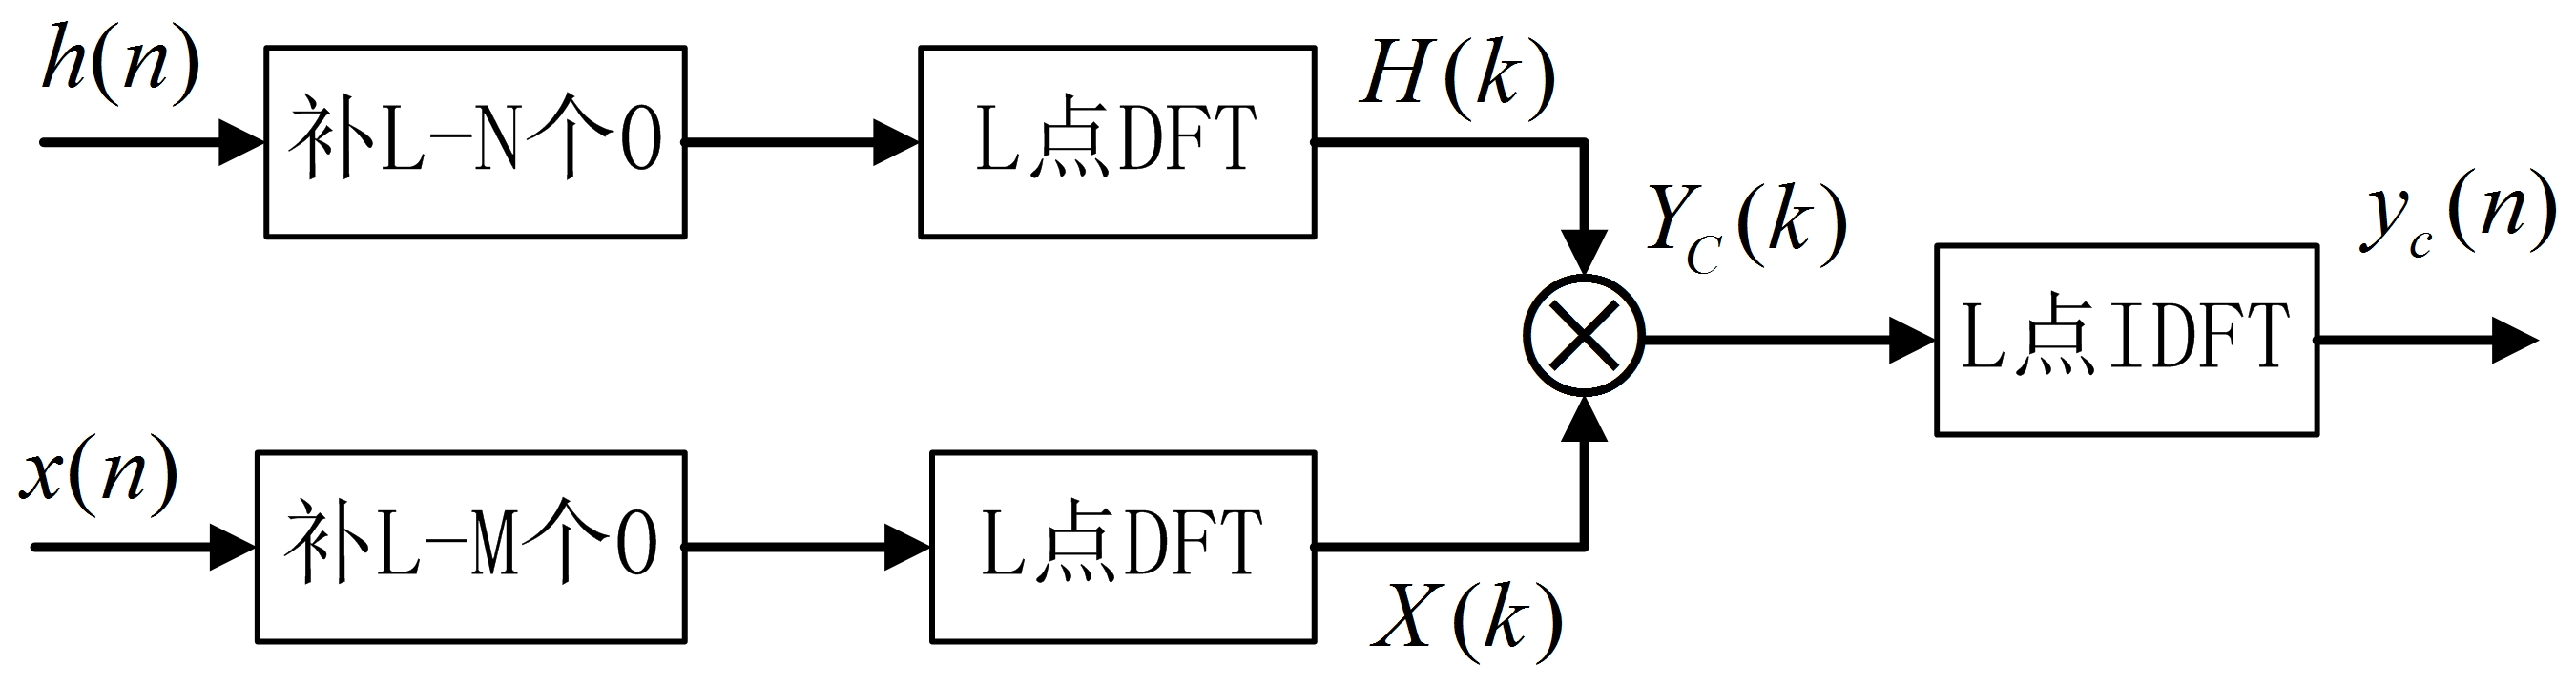
\includegraphics[width=0.99\linewidth]{jisuanxunhuanjuanji.jpg}
  \end{figure}  
  注意:这里需要做3次$DFT$计算,为何?因为$DFT$有快速算法$FFT$,可大大加快计算速度。
\end{frame}
%
\begin{frame}[shrink]\frametitle{长序列卷积计算}%[allowframebreaks]
(2)长序列卷积计算

\begin{enumerate}
  \item \textbf{问题:}\par
         在实践中经常两个序列的长度相差很大,如$M\gg N$,利用卷积定理计算时需补0,这样造成存储空间和计算能力的浪费。\par
         而且在某些应用中,序列长度不定或者被认为是无限长。
  \item \textbf{解决方法:} 将长序列分段计算。  \par
%        设$h(n)$长度为$N$,$x(n)$无限长,可通过分段处理,设每段长度为$M$,可令:
%        $$x(n) = \sum_{k=0}^{\infty}x_k(n) \quad\mbox{则:}\quad  x_k(n) = x(n)\cdot R_M(n-kM)$$
%        可举一例。
\end{enumerate}
\end{frame}

\begin{frame}[shrink]\frametitle{长序列卷积计算的公式}%[allowframebreaks]
 设$h(n)$长度为$N$,$x(n)$无限长,可通过分段处理,设每段长度为$M$,可令:
$$x(n) = \sum_{k=0}^{\infty}x_k(n) \quad\mbox{则:}\quad  x_k(n) = x(n)\cdot R_M(n-kM)$$
%可举一例。:
%        $$x(n) = \sum_{k=0}^{\infty}x_k(n) \quad\quad\quad  x_k(n) = x(n)\cdot R_M(n-kM)$$
          \begin{equation*}
            \begin{split}
            y(n)    &= h(n)* x(n) = h(n) * \left[  \sum_{k=0}^{\infty}x_k(n)  \right]\\
                    &=  \sum_{k=0}^{\infty}  h(n) * x_k(n)  \\
                    &=  \sum_{k=0}^{\infty}  y_k(n)  \quad\quad\mbox{这里:} y_k(n)= h(n)* x_k(n)
            \end{split}
          \end{equation*}
\end{frame}

\begin{frame}[shrink]\frametitle{举例说明}%[allowframebreaks]
   例如,设 $N=3,M=5,L = N+M-1=7$
 %       \quad\newline\newline\newline\newline\newline\newline\newline\newline\newline\newline\newline\newline\quad


        \begin{equation*}
            \begin{split}
        \mbox{则:}\quad    y(n) &= y_0(n)+y_1(n)+y_2(n)+ \cdots y_k(n)+ \cdots
                   \quad\quad\quad\quad\quad\quad\quad\quad\quad\quad\\
                 &= \sum_{k=0}^{\infty}  y_k(n)
            \end{split}
          \end{equation*}
          计算过程
          \begin{enumerate}
            \item [1] 先后计算$y_0(n),y_1(n),y_2(n), \cdots y_k(n), \cdots$
            \item [2] 分别相加。
          \end{enumerate}

\end{frame}
%
%
%
%
%\newpage
\subsection{用$DFT$对信号进行谱分析}
\begin{frame}[shrink]\frametitle{信号的谱分析}%[allowframebreaks]
\begin{dablock}
所谓信号的谱分析,就是计算信号的傅里叶变换。对于连续信号和系统,可以通过时域采样,应用DFT进行近似谱分析。
\end{dablock}


\textbf{一、用$DFT$对连续信号进行谱分析}

   用DFT对连续信号进行谱分析必然是近似的,其近似程度与信号带宽、采样频率和截取长度有关。

\end{frame}



\begin{frame}[shrink]\frametitle{用$DFT$对连续信号进行谱分析}%[allowframebreaks]

\begin{enumerate}
  \item [(1)]  问题 \par
        给定有限长带限信号$x_a(t)$,如何得到$X_a(jf)$\newline


  \item [(2)]   谱分析的过程:
        $$x_a(t) \longrightarrow  x(n) \longrightarrow X(k) \longrightarrow X_a(jf)$$
\end{enumerate}
\end{frame}


%\begin{frame}[shrink]\frametitle{谱分析的过程}%[allowframebreaks]
%hahaha
%
%\end{frame}

\begin{frame}[shrink]\frametitle{}%[allowframebreaks]
\begin{enumerate}
	\item [(3)]采样参数的说明\par

        \qquad 用DFT对连续信号进行谱分析必然是近似的,其近似程度与信号带宽、采样频率和截取长度有关。因此采样参数与上述三者相关。
        \begin{equation*} %\label{fol2218}
            \left. \begin{aligned}
                T   \quad   &: \mbox{采样间隔}\\
                f_s \quad   &: \mbox{采样频率}\\
            \end{aligned}  \right\}
            \qquad\qquad   T = \frac{1}{f_s},\quad f_s = \frac{1}{T}    % \right.
            \qquad \qquad\qquad\qquad\quad
        \end{equation*}
        \begin{equation*} %\label{fol2218}
            \left. \begin{aligned}
                N   \quad   &: \mbox{采样点数}\\
                T_p \quad   &: \mbox{信号长度}\\
            \end{aligned}  \right\}
            \qquad\qquad  T_p  =  NT,\quad  N = \frac{T_p}{T}    % \right.
            \qquad \qquad\qquad\qquad
        \end{equation*}
\end{enumerate}        
\end{frame}




%\begin{frame}[shrink]\frametitle{title}%[allowframebreaks]
%
%图示
%\end{frame}



\begin{frame}[shrink]\frametitle{}%[allowframebreaks]
\begin{enumerate}
	\item [(4)]参数之间的关系 
\end{enumerate}      
  
  
  
        \qquad 在2.4节中,我们有 $X(e^{j\omega})=\hat{X}_a(j\Omega)\big|_{\omega = \Omega T}$,则有:
        $$X(e^{j\omega})=X_a(j\Omega)\big|_{\omega = \Omega T} =X_a(jf)\big|_{\omega = 2\pi fT}$$
        \begin{equation*}
        \begin{split}
        \because\qquad\quad \omega      &= \Omega T = 2\pi f T =2\pi T f  %= \frac{2\pi}{f_s} f
           \qquad\qquad    \big(\Omega = 2\pi f \big)  \qquad\qquad\qquad\qquad\qquad\\
        \therefore\qquad   \Delta\omega &=  2\pi T\Delta f  \qquad\qquad\qquad\qquad\quad\;    \big(\Delta\omega = \frac{2\pi}{N}\big)\\
        \therefore\qquad   \Delta f     &=  \frac{1}{2\pi T} \Delta\omega 
                                         =  \frac{1}{2\pi T}\cdot \frac{2\pi}{N} = \frac{1}{NT}
        \end{split}
        \end{equation*}
        令$F=\Delta f$,这里$F$称为频率分辨率,表示对模拟信号频谱的采样间隔。
        $$\mbox{\textbf{结论:}} \qquad\qquad F= \frac{1}{NT} = \frac{1}{T_p}
           \qquad\qquad\qquad\qquad\qquad\qquad\qquad\qquad$$
\end{frame}
  %\item



\begin{frame}[shrink]\frametitle{}%[allowframebreaks]

问题在于怎么用$X(k)$表示$X_a(jf)$
$$\because\qquad X(k) \quad =  X\left(e^{j\omega}\right)\big|_{\omega = \frac{2\pi}{N} k}   \quad\mbox{且}\quad
X\left(e^{j\omega}\right) =  \hat{X}_a(j\Omega)\big|_{ \omega = \Omega T }  \qquad\qquad\qquad $$
\begin{equation*}
\begin{split}
X(k) \quad&=  \hat{X}_a(j\Omega)\big|_{ \Omega T =\frac{2\pi}{N} k  }   \quad \\
          &=  \hat{X}_a(j\Omega)\big|_{ 2\pi f T =\frac{2\pi}{N} k  } \\
          &=  \hat{X}_a(j\Omega)\big|_{ f  =\frac{1}{NT} k  } \quad\\
          &=  \hat{X}_a(j\Omega)\big|_{ f  =k F  }   \qquad\quad  (F= \frac{1}{NT})\\
          &=  \frac{1}{T}\sum_{m=-\infty}^{\infty}X_a\left(j\Omega-j m\Omega_s\right)\Big|_{ f  = k F  }   \\
%          &=  \frac{1}{T} X_a\left(j\Omega\right)\Big|_{ f  = k F  }     \qquad\qquad  k = 0,1,\cdots ,N-1  \\
%          &=  \frac{1}{T} X_a\left(j 2\pi f\right)\Big|_{ f  = k F  }     \qquad\quad  k = 0,1,\cdots ,N-1\\
%          &\quad  \qquad\mbox{令:}X_a(kf) = X_a\left(j 2\pi f\right)\big|_{ f  = k F  }  \qquad\quad k = 0,1,\cdots ,N-1 \\
%\therefore\qquad X(k)     
%         &=  \frac{1}{T} X_a(kf)    \qquad\qquad k = 0,1,\cdots ,N-1\\
%\therefore\quad X_a(kf)   
%         &= T\cdot X(k)             \;\qquad\qquad k = 0,1,\cdots ,N-1
\end{split}
\end{equation*}
\end{frame}





\begin{frame}[shrink]\frametitle{}%[allowframebreaks]
接着前面的公式,继续推导,前述有:
\begin{equation*}
\begin{split}
X(k) \quad  &=  \frac{1}{T}\sum_{m=-\infty}^{\infty}X_a\left(j\Omega-j m\Omega_s\right)\Big|_{ f  = k F  }  \qquad\qquad\qquad\qquad\qquad\qquad\qquad\qquad \\
			&=  \frac{1}{T} X_a\left(j\Omega\right)\Big|_{ f  = k F  }     \qquad\quad  k = 0,1,\cdots ,N-1  \\
			&=  \frac{1}{T} X_a\left(j 2\pi f\right)\Big|_{ f  = k F  }     \qquad  k = 0,1,\cdots ,N-1\\
	\quad   &\quad   \quad  \\
\qquad\mbox{令}X_a(kf) =
			&\quad   X_a\left(j 2\pi f\right)\big|_{ f  = k F  }  \qquad\quad k = 0,1,\cdots ,N-1 \\
\therefore\qquad X(k)     
			&=  \frac{1}{T} X_a(kf)    \qquad\qquad k = 0,1,\cdots ,N-1\\
\therefore\quad X_a(kf)   
			&= T\cdot X(k)             \;\qquad\qquad k = 0,1,\cdots ,N-1
\end{split}
\end{equation*}
\end{frame}



\begin{frame}[shrink]\frametitle{谱分析步骤}%[allowframebreaks]

\begin{enumerate}
	\item [(5)] 谱分析步骤
\end{enumerate}  
  
        \begin{enumerate}
          \item 对$x_a(t)$采样,得到有限长$x(n)$,长度为$N$。
          \item 计算$DFT$,$\quad x(n)\longleftrightarrow X(k)$
          \item $X_a(kf)   = T\cdot X(k)   \qquad\qquad 0\leq k \leq N-1$
        \end{enumerate}

 % \item
\end{frame}

\begin{frame}[shrink]\frametitle{采样参数的选择}%[allowframebreaks]
  
\begin{enumerate}
	\item [(6)] 采样参数的选择
\end{enumerate}   
        %用$DFT$对连续信号进行谱分析必然是近似的,其近似程度与信号带宽、采样频率和截取长度有关。因此采样参数与上述三者相关。
        在对连续信号进行谱分析是,主要关心两个问题
        \begin{enumerate}
          \item 谱分析范围: \qquad 决定信号带宽
          \item 频率分辨率: \qquad 决定信号长度
        \end{enumerate}

        问题:
        \begin{itemize}
          \item 已知信号频率分辨率$F$,信号最高频率$f_c$,
          \item 确定谱分析参数。
          \begin{enumerate}
          	\item  [(a)]最小记录时间$T_{p\: min}$
          	\item  [(b)]最大采样周期 $T_{max}$
          	\item  [(c)]最小采样点数$N_{min}$
        \end{enumerate}
        \end{itemize}
\end{frame}




\begin{frame}[shrink]\frametitle{谱分析参数}%[allowframebreaks]
        \begin{enumerate}
          \item 最小记录时间$T_{p\: min}$
            $$F=\frac{1}{T_p} \quad \Longrightarrow\quad  T_p=\frac{1}{F}  \quad \Longrightarrow\quad   T_p\geq \frac{1}{F_{max}}$$
            $$\therefore\qquad T_{p\:min} = \frac{1}{F_{max}}\qquad\qquad\qquad\qquad\qquad$$
          \item 最大采样周期 $T_{max}$
            $$f_s \geq 2f_c \quad \Longrightarrow\quad \frac{1}{T} \geq 2f_c \quad\Longrightarrow\quad T\leq \frac{1}{2f_c} $$
            $$\therefore\qquad T_{max} = \frac{1}{2f_c}\qquad\qquad\qquad\qquad\qquad$$
          \item 最小采样点数$N_{min}$
            $$\therefore\qquad N_{min} = \frac{T_{p\: min}}{T_{max}}\qquad\qquad\qquad\qquad\qquad$$
        \end{enumerate}
%\end{enumerate}
\end{frame}

\begin{frame}[shrink]\frametitle{举例说明}%[allowframebreaks]
\begin{example}
对实信号做谱分析,要求谱分辨率$F\leq10Hz$,信号最高频率为$f_c = 2.5kHz$。
试确定最小记录时间$T_{p\: min}$,最小记录点数$N_{min}$,最大采样周期$T_{max}$。	
\end{example}
%\textbf{例:}
%
%
\textbf{解:}
\begin{equation*}
\begin{split}
    T_{p\:min} &= \frac{1}{F_{max}}   =  \frac{1}{10} =0.1\:s \quad\qquad\qquad\qquad\qquad\qquad   \\
    T_{max}    &= \frac{1}{2f_c} \quad     =  \frac{1}{5000} =0.2\:ms               \\
    N_{min}    &= \frac{T_{p\: min}}{T_{max}}  = \frac{0.1s}{02.ms}  = 500
\end{split}
\end{equation*}
\end{frame}


\begin{frame}[shrink]\frametitle{用$DFT$对离散序列做谱分析}%[allowframebreaks]   \end{frame}
\textbf{二、用$DFT$对序列做谱分析}
\begin{enumerate}
  \item 有限长序列\par
        \qquad 设有限长序列$x(n)$长度为$N$,则$X(k)$是$X(e^{j\omega})$ 在$[0,2\pi]$上的$N$点等间隔采样,直接得到。
        频率分辨率就是采样间隔$\frac{2\pi}{N} $。
        序列的FT可以利用DFT来计算。
  \item 周期序列$\tilde{x}(n) = x((n))_N$

\end{enumerate}
\end{frame}



\begin{frame}[shrink]\frametitle{周期序列$\tilde{x}(n) = x((n))_N$}%[allowframebreaks]


  \begin{enumerate}
    \item [方法1]利用公式直接得到
  \end{enumerate}
      $$ X(e^{j\omega}) =FT[\tilde{x}(n)] = \frac{2\pi}{N}\sum_{k=-\infty}^{\infty}\tilde{X}(k)\delta(\omega-\frac{2\pi}{N}k)$$
      其强度为$\frac{2\pi}{N}\tilde{X}(k)$,为周期为$N$ 的周期序列,只需要知道$\tilde{X}(k)$,就可以得到$FT[\tilde{x}(n)]$,而$\tilde{X}(k) = DFS[\tilde{x}(n)]$。\par
      \textbf{步骤:}
      \begin{enumerate}
        \item 取主值,$x(n) = x(n)R_N(n)$
        \item 做$DFT$变换,$X(k) = DFT[x(n)]$
        \item 延拓,$\tilde{X}(k) = X((n))_N$
        \item 代公式
      \end{enumerate}
    
\end{frame}




\begin{frame}[shrink]\frametitle{周期序列$\tilde{x}(n) = x((n))_N$}%[allowframebreaks]
\begin{enumerate}
	\item [方法2]截取$\tilde{x}(n)$的整数个周期进行DFT,可得到其频谱结构,达到谱分析的目的。


    截取$\tilde{x}(n)$的$m$个周期,设其长度为M,即
    $$X_M(n) = \tilde{x}(n)R_M(n)\qquad\qquad  (M=mN,m\in Z)$$
    $$\mbox{设}\qquad x_M(n)\longleftrightarrow X_M(k)\qquad\qquad (0\leq k \leq mN-1)$$
    则
%    有:
%    \begin{equation*}
%    X_M(k)=
%    \left\{\begin{array}{r@{,\quad}l}
%    mX\Big(\frac{k}{m}\Big)  &   \mbox{$\frac{k}{m}$为整数}\\
%    0                        &   \mbox{$\frac{k}{m}$不为整数}
%    \end{array} \right.
%    \end{equation*}
    $ X_M(k) $也能表示$ \tilde{x}(n) $的频谱结构。
\end{enumerate}    
\end{frame}    
    
\begin{frame}[shrink]\frametitle{下面推导$X(k)$与$X_M(k)$的关系。}%[allowframebreaks]    
截取$\tilde{x}(n)$的$m$个周期,设其长度为M,即
$$X_M(n) = \tilde{x}(n)R_M(n)\qquad\qquad  (M=mN,m\in Z)$$
$$\mbox{设}\qquad x_M(n)\longleftrightarrow X_M(k)\qquad\qquad (0\leq k \leq mN-1)$$
    下面给出$X(k)$与$X_M(k)$的关系。
  \begin{lemma}
    \begin{equation*}
    \sum_{n=0}^{mN-1}f(n) = \sum_{r=0}^{m-1}\sum_{n'=0}^{N-1}f(n'+rN) \qquad\mbox{设$f(n)$的周期为$N$}
    \end{equation*}
  \end{lemma}
\end{frame} 

\begin{frame}[shrink]\frametitle{}%[allowframebreaks]  
    \begin{equation*}
    \begin{split}
    X_M(k) &=  \sum_{n=0}^{mN-1}x_M(n) e^{-j\frac{2\pi}{M} kn  }   \qquad   
            =  \sum_{n=0}^{mN-1}\tilde{x}(n) e^{-j\frac{2\pi}{M} kn  }   \qquad   \\
           &=  \sum_{r=0}^{m-1}\sum_{n'=0}^{N-1}\tilde{x}(n'+rN) e^{-j\frac{2\pi}{M} k(n'+rN)  }   \qquad \left(n\rightarrow n'+rN  \right)   \\
           &=  \sum_{r=0}^{m-1}\left[\sum_{n'=0}^{N-1}\tilde{x}(n'+rN) e^{-j\frac{2\pi}{M} kn'} \right]  e^{-j\frac{2\pi}{M} krN  }  \\
           &=  \sum_{r=0}^{m-1}\left[\sum_{n'=0}^{N-1}\tilde{x}(n') e^{-j\frac{2\pi}{N}\frac{k}{m}n'}\right] e^{-j\frac{2\pi}{m} kr} \qquad (M=mN)   \\
           &= \sum_{r=0}^{m-1} X\Big(\frac{k}{m}\Big)\cdot e^{-j\frac{2\pi}{m} kr} \\
           &=  X\Big(\frac{k}{m}\Big)\cdot \sum_{r=0}^{m-1}e^{-j\frac{2\pi}{m} kr}
    \end{split}
    \end{equation*}
%    而:
%    \begin{equation*}
%    \sum_{r=0}^{m-1}e^{-j\frac{2\pi}{m} kr} = \sum_{r=0}^{m-1}\left[e^{-j\frac{2\pi}{m} k}\right]^r=
%    \left\{\begin{array}{r@{,\quad}l}
%    m  &   \mbox{$\frac{k}{m}$ 为整数}\\
%    0  &   \mbox{$\frac{k}{m}$ 不为整数}
%    \end{array} \right.
%    \end{equation*}
\end{frame}

\begin{frame}[shrink]\frametitle{下面推导$X(k)$与$X_M(k)$的关系。}%[allowframebreaks] 
因为:
$$X_M(k)  =  X\Big(\frac{k}{m}\Big)\cdot \sum_{r=0}^{m-1}e^{-j\frac{2\pi}{m} kr} $$
    而:
    \begin{equation*}
    \sum_{r=0}^{m-1}e^{-j\frac{2\pi}{m} kr} = \sum_{r=0}^{m-1}\left[e^{-j\frac{2\pi}{m} k}\right]^r=
    \left\{\begin{array}{r@{,\quad}l}
    m  &   \mbox{$\frac{k}{m}$ 为整数}\\
    0  &   \mbox{$\frac{k}{m}$ 不为整数}
    \end{array} \right.
    \end{equation*}
    所以有,
    \begin{equation*}
    X_M(k)=
    \left\{\begin{array}{r@{,\quad}l}
    mX\Big(\frac{k}{m}\Big)  &   \mbox{$\frac{k}{m}$为整数}\\
    0                        &   \mbox{$\frac{k}{m}$不为整数}
    \end{array} \right.
    \end{equation*}
\end{frame}





\begin{frame}[shrink]\frametitle{举例说明:$ x(n)见板书 $}%[allowframebreaks]
%    例: 
    设$N=4$,取$m=3$,则$M=mN= 12$.
    \begin{equation*}
    X_M(k)= X_{12}(k)=
    \left\{\begin{array}{r@{,\quad}l}
    3 X\Big(\frac{k}{3}\Big)  &   \mbox{$\frac{k}{m}$为整数}\\
    0                        &   \mbox{$\frac{k}{m}$不为整数}
    \end{array} \right.
    \end{equation*}
    则$X_M(k)= X_{12}(k)$为:
    $$
        \begin{array}{lll}
        X_{12}(0) = 3X(\frac{0}{3}) = 3   &   \qquad X_{12}(1) = 0  &   X_{12}(2) = 0  \qquad\qquad\qquad\qquad\\
        X_{12}(3) = 3X(\frac{3}{3}) = 4.5 &   \qquad X_{12}(4) = 0  &   X_{12}(5) = 0 \\
        X_{12}(6) = 3X(\frac{6}{3}) = 6   &   \qquad X_{12}(7) = 0  &   X_{12}(8) = 0 \\
        X_{12}(9) = 3X(\frac{9}{3}) = 7.5 &   \qquad X_{12}(10) = 0  &   X_{12}(11) = 0 \\
        \end{array}
    $$



    \textbf{注:}
    由此可见,$X_M(k)$也能代表$\tilde{x}(n)$的频谱结构,只是当$k=rm$时,有$X_M(rm)= mX(r)$。因此只要截取$\tilde{x}(n)$的整数倍周期做$DFT$,就可以得到它的频率结构进行谱分析。


\end{frame}


\subsection{用DFT进行谱分析的误差问题}
\begin{frame}[shrink]\frametitle{用DFT进行谱分析的误差问题}%[allowframebreaks]

 实际应用中,DFT用于对连续信号做谱分析时,需对其进行截断和采样,其必将引起某些误差。
\begin{enumerate}
  \item 混叠现象
  \item 栅栏效应
  \item 截断效应
\end{enumerate}

\end{frame}
%
%
\begin{frame}[shrink]\frametitle{混叠现象}%[allowframebreaks]

 混叠现象  \par
     \begin{enumerate}
       \item  在$x_a(t)$进行采样时,存在采样定理的限制,
              $$f_s \geq 2 f_c\quad\qquad\qquad\qquad\qquad\qquad$$
              否则将在$\omega = \pi\quad\:$$(f=\frac{f_s}{2})$ 处存在一个频率混叠的问题。
       \item  措施:\par
              采样之前进行预滤波,滤除高于折叠频率$\frac{f_s}{2}$ 的频率成分,避免频率混叠现象。
     \end{enumerate}
\end{frame}
%
%
%
\begin{frame}[shrink]\frametitle{栅栏效应}%[allowframebreaks]
 栅栏效应
     \begin{enumerate}
       \item  N点DFT$X(k)$是对$X(e^{j\omega})$在$[0,2\pi]$ 上的$N$点等间隔采样,仅能得到连续频谱的N个采样点,采样点之间的频率看不到。这种现象称为栅栏效应。
       \item  措施:\par 为使得栅栏变细,可加大采样点数,对有限长序列来说,可在原序列尾部补0。
              采样之前进行预滤波,滤除高于折叠频率$\frac{f_s}{2}$ 的频率成分,避免频率混叠现象。
     \end{enumerate}
\end{frame}
%
%
%
%
\begin{frame}[shrink]\frametitle{截断效应}%[allowframebreaks]
   截断效应  \qquad(自己看)
  \begin{enumerate}
    \item 泄露
    \item 谱间干扰
  \end{enumerate}

\end{frame}


\end{document}

